% ==============================================================================
% Template de Relatório — Seminários em Engenharia Mecânica (MEM)
% Departamento de Engenharia Mecânica, Universidade de Aveiro
% ==============================================================================
\documentclass[11pt,a4paper]{article}

% ==============================================================================
% Configurações Gerais do Template — Seminários em Engenharia Mecânica (DEM@UA)
% ==============================================================================

% --- Codificação e Idioma ---
\usepackage[utf8]{inputenc}
\usepackage[T1]{fontenc}
\usepackage[portuguese]{babel}
\usepackage{textcomp}
\usepackage{microtype}

% --- Tipografia: Apenas DUAS fontes ---
% 1) Corpo de texto (serif): Charter
% 2) Capa, títulos, cabeçalhos, rodapés e tabelas (sans-serif): Roboto
\usepackage{charter}
\usepackage{roboto}

% --- Margens e Espaçamento ---
\usepackage[
  a4paper,
  top=2.5cm,
  bottom=2.5cm,
  left=2.5cm,
  right=2.5cm,
  headheight=22pt
]{geometry}
\linespread{1.15}
\setlength{\parindent}{0pt}
\setlength{\parskip}{6pt}

% --- Paleta de Cores (Tons neutros + verde institucional UA/DEM, sem azulados) ---
\usepackage[table]{xcolor}
\definecolor{uagreen}{HTML}{6BA61E}      % Verde institucional DEM/UA
\definecolor{uadark}{HTML}{222222}       % Grafite neutro escuro para títulos e destaque
\definecolor{uamuted}{HTML}{595959}      % Cinzento neutro médio para rodapés/legendas
\definecolor{ualightbg}{HTML}{F7F7F7}    % Cinzento neutro muito claro para caixas
\definecolor{uatablehead}{HTML}{EBEBEB}  % Cinzento neutro suave para cabeçalhos de tabela
\definecolor{uaborder}{HTML}{D4D4D4}     % Cinzento neutro para linhas de separação

% --- Matemática e Números (separador decimal PT) ---
\usepackage{amsmath, amssymb}
\usepackage{icomma}

% --- Figuras, Tabelas e Listas ---
\usepackage{graphicx}
\graphicspath{{figs/}}
\usepackage{float}
\usepackage{booktabs}
\usepackage{tabularx}
\usepackage{array}
\usepackage{enumitem}
\usepackage[font={small,sf}, labelfont={bf,color=uadark}, skip=6pt]{caption}

% Espaçamento vertical confortável nas tabelas
\renewcommand{\arraystretch}{1.35}
\newcolumntype{L}[1]{>{\raggedright\arraybackslash}p{#1}}
\newcolumntype{R}[1]{>{\raggedleft\arraybackslash}p{#1}}
\newcolumntype{Y}{>{\raggedright\arraybackslash}X}

% --- Hierarquia de Títulos (Roboto, maiores do que o texto 11pt) ---
\usepackage{titlesec}

\titleformat{\section}
  {\sffamily\LARGE\bfseries\color{uadark}}
  {\textcolor{uagreen}{\thesection}}{0.6em}{}
  [\vspace{2pt}{\color{uagreen}\titlerule[1.2pt]}]
\titlespacing*{\section}{0pt}{22pt}{10pt}

\titleformat{\subsection}
  {\sffamily\Large\bfseries\color{uadark}}
  {\textcolor{uagreen}{\thesubsection}}{0.5em}{}
\titlespacing*{\subsection}{0pt}{16pt}{6pt}

\titleformat{\subsubsection}
  {\sffamily\large\bfseries\color{uamuted}}
  {\textcolor{uagreen}{\thesubsubsection}}{0.5em}{}
\titlespacing*{\subsubsection}{0pt}{12pt}{4pt}

% --- Cabeçalhos e Rodapés ---
\usepackage{fancyhdr}
\usepackage{lastpage}
\pagestyle{fancy}
\fancyhf{}
\fancyhead[L]{\sffamily\footnotesize\color{uamuted}Seminários em Engenharia Mecânica \textbar{} DEM -- UA}
\fancyhead[R]{\sffamily\footnotesize\color{uamuted}\nouppercase{\leftmark}}
\fancyfoot[L]{\sffamily\footnotesize\color{uamuted}Mestrado em Engenharia Mecânica 2026/2027}
\fancyfoot[R]{\sffamily\footnotesize\color{uadark}\textbf{\thepage} / \pageref{LastPage}}
\renewcommand{\headrulewidth}{0.4pt}
\renewcommand{\headrule}{\hbox to\headwidth{\color{uaborder}\leaders\hrule height \headrulewidth\hfill}}
\renewcommand{\footrulewidth}{0pt}

\fancypagestyle{frontmatter}{
  \fancyhf{}
  \fancyhead[L]{\sffamily\footnotesize\color{uamuted}Seminários em Engenharia Mecânica \textbar{} DEM -- UA}
  \fancyhead[R]{\sffamily\footnotesize\color{uamuted}\nouppercase{\leftmark}}
  \fancyfoot[L]{\sffamily\footnotesize\color{uamuted}Mestrado em Engenharia Mecânica 2026/2027}
  \fancyfoot[R]{\sffamily\footnotesize\color{uadark}\textbf{\thepage}}
  \renewcommand{\headrulewidth}{0.4pt}
  \renewcommand{\headrule}{\hbox to\headwidth{\color{uaborder}\leaders\hrule height \headrulewidth\hfill}}
  \renewcommand{\footrulewidth}{0pt}
}

% --- Caixa Moderna de Conteúdo (quebra automaticamente entre páginas) ---
\usepackage[most]{tcolorbox}
\newtcolorbox{campotexto}{
  breakable,
  enhanced,
  colback=ualightbg,
  colframe=ualightbg,
  borderline west={2.5pt}{0pt}{uagreen},
  boxrule=0pt,
  arc=2pt,
  left=10pt,
  right=10pt,
  top=8pt,
  bottom=8pt,
  before skip=6pt,
  after skip=10pt
}

% Estilo discreto para texto de orientação (substituir pelo conteúdo final)
\newcommand{\instrucao}[1]{\leavevmode{\color{uamuted}\itshape #1}}

% --- Bibliografia (BibTeX / natbib, estilo numérico) ---
\usepackage[numbers,sort&compress]{natbib}
\renewcommand{\bibsection}{}
\setlength{\bibsep}{4pt}

% --- Gráficos Vetoriais (para a Capa) ---
\usepackage{tikz}
\usetikzlibrary{calc}

% --- Hiperligações e Metadados PDF (sem cores azuladas) ---
\usepackage[
  colorlinks=true,
  linkcolor=uadark,
  urlcolor=uagreen,
  citecolor=uagreen,
  pdfborder={0 0 0}
]{hyperref}
\urlstyle{sf}

% --- Comandos para Metadados do Relatório ---
\newcommand{\tituloProjeto}{Título do Projeto de Inovação e I\&D}
\newcommand{\acronimoProjeto}{ACRÓNIMO}
\newcommand{\numeroGrupo}{Grupo \#}
\newcommand{\anoLetivo}{2026/2027}


% ------------------------------------------------------------------------------
% IDENTIFICAÇÃO DO PROJETO (atualizar aqui para refletir na capa)
% ------------------------------------------------------------------------------
\renewcommand{\tituloProjeto}{Beyond Wheels}
\renewcommand{\acronimoProjeto}{BW}
\renewcommand{\numeroGrupo}{Grupo 3}
\renewcommand{\anoLetivo}{2026/2027}

% ==============================================================================
\begin{document}

% --- Capa ---
% ==============================================================================
% Capa do Relatório (design limpo e moderno, apenas com a fonte sans-serif)
% ==============================================================================
\begin{titlepage}
\thispagestyle{empty}

% Faixa vertical lateral subtil (identidade UA / DEM)
\begin{tikzpicture}[remember picture, overlay]
  \fill[uadark] (current page.north west) rectangle ([xshift=1.1cm]current page.south west);
  \fill[uagreen] ([xshift=1.1cm]current page.north west) rectangle ([xshift=1.35cm]current page.south west);
\end{tikzpicture}

\sffamily
\hspace*{0.8cm}%
\begin{minipage}[t][0.94\textheight][t]{0.92\textwidth}

  % Logótipo institucional UA / DEM
  \vspace*{0.4cm}
  \noindent
\includegraphics[width=0.72\textwidth]{UA_DEM_vertical2.pdf}

  \vspace{2.8cm}

  % Identificação da Unidade Curricular
  {\large\bfseries\color{uagreen} SEMINÁRIOS EM ENGENHARIA MECÂNICA}\\[0.35cm]
  {\normalsize\color{uamuted} Mestrado em Engenharia Mecânica \textbar{} \anoLetivo}

  \vspace{0.9cm}
  \noindent\textcolor{uagreen}{\rule{3.5cm}{2pt}}
  \vspace{0.9cm}

  % Título Principal
  {\fontsize{26}{32}\selectfont\bfseries\color{uadark} Relatório Final\par}
  \vspace{0.35cm}
  {\Large\color{uamuted} Proposta de projeto de inovação, investigação e desenvolvimento -- Ac5\par}

  \vspace{1.4cm}

  % Bloco de identificação do projeto
  \begin{tcolorbox}[
    colback=ualightbg,
    colframe=uaborder,
    boxrule=0.5pt,
    arc=3pt,
    left=14pt, right=14pt, top=12pt, bottom=12pt
  ]
    {\small\bfseries\color{uagreen} PROJETO \textbar{} \acronimoProjeto}\\[0.25cm]
    {\Large\bfseries\color{uadark} \tituloProjeto}\\[0.25cm]
    {\normalsize\color{uamuted} \numeroGrupo}
  \end{tcolorbox}

  \vspace{1.8cm}

  % Autores
  {\small\bfseries\color{uagreen} AUTORES}\\[0.35cm]
  {\normalsize\color{uadark}
    Diana Baldaia - N.º Mec: 113112\\[0.15cm]
    Leandro Simões - N.º Mec: 107262\\[0.15cm]
    Marco Pereira - N.º Mec: 130641\\[0.15cm]
    Mariana Lobo - N.º Mec: 114073\\[0.15cm]
    Rafael Alegria - N.º Mec: 113701\\[0.15cm]
    Simão Pires - N.º Mec: 113531
  }

  \vfill

  % Rodapé da capa
  \noindent\textcolor{uaborder}{\rule{\textwidth}{0.5pt}}\\[0.3cm]
  {\small\color{uamuted} Universidade de Aveiro \hfill \anoLetivo}

\end{minipage}
\end{titlepage}


% --- Índice ---
\newpage
\pagestyle{frontmatter}
\pagenumbering{roman}
{\setlength{\parskip}{1pt}\tableofcontents}
\newpage
\pagestyle{fancy}
\pagenumbering{arabic}

% --- Secções do Relatório ---
\section{Introdução}
\label{sec:intro}
% ==============================================================================
% Secção 1: Introdução
% ==============================================================================

\subsection{Título do projeto (em português)}
\begin{campotexto}
Otimização do Carro do Futuro (Beyond Wheels)
\end{campotexto}

\subsection{Título do projeto (em inglês)}
\begin{campotexto}
Future Cars Optimization (Beyond Wheels)
\end{campotexto}

\subsection{Acrónimo}
\begin{campotexto}
BW
\end{campotexto}

\subsection{Palavras-chave (em português)}
\begin{campotexto}
Bateria de Lítio, Bateria de Sódio, Suspensão Adaptativa, Regeneração de Energia
\end{campotexto}

\subsection{Palavras-chave (em inglês)}
\begin{campotexto}
Lithium Battery, Sodium Battery, Adaptive Suspension, Energy Regeneration
\end{campotexto}

\subsection{Áreas científicas principais}
\begin{campotexto}
Engenharia Mecânica, Eletrónica
\end{campotexto}

\subsection{Duração em meses}
\begin{campotexto}
36
\end{campotexto}

\subsection{Identificação de questões éticas}
\begin{campotexto}
As questões éticas do BeyondWheels resultam sobretudo do impacto ambiental e
social das tecnologias estudadas e da segurança de quem utiliza os veículos.
No armazenamento de energia, a transição das baterias de lítio para baterias de
sódio e a sua reciclagem no fim de vida respondem a preocupações éticas e
ambientais associadas à extração de lítio, ao descarte de baterias e ao risco de
incêndio. É assim necessário garantir que a cadeia de valor dos materiais e o
tratamento das baterias usadas sejam sustentáveis e responsáveis.

A suspensão adaptativa e preditiva, baseada em sensores e Inteligência
Artificial, atua diretamente sobre a estabilidade e o conforto do veículo.
Decisões incorretas ou falhas do sistema podem, por isso, afetar a segurança de
passageiros e de outros utilizadores da estrada, o que exige validação rigorosa,
modos de funcionamento seguro em caso de falha e conformidade com a
regulamentação e a certificação de segurança europeias. Por recolher e
processar dados em tempo real sobre o veículo e a via, o sistema levanta ainda
questões de privacidade e de proteção de dados, devendo respeitar o RGPD e ser
transparente quanto aos dados recolhidos, à sua finalidade e às decisões
tomadas pelo modelo.
\end{campotexto}

\subsection{Caracterização dos proponentes}
\begin{campotexto}
Nesta secção apresenta-se a equipa proponente do projeto BeyondWheels, com as
suas competências, funções e contributos para o desenvolvimento da proposta. O
projeto é interdisciplinar, ao integrar mecânica, eletrónica, materiais e
sustentabilidade e modelos de Inteligência Artificial. A
equipa foi, por isso, organizada por funções, cada uma associada a um conjunto
de atividades distinto: a definição do método das suspensões adaptativas, a
regeneração de energia, a transição das baterias de lítio para sódio, a
autonomia e reciclagem das baterias, o orçamento e a comunicação do projeto
através da página web.

O projeto desenvolve-se em consórcio com dois outros grupos, que colaboram de
forma localizada em atividades específicas, mantendo o Grupo 3 a coordenação e
a responsabilidade pela proposta:
\begin{itemize}
  \item \textbf{Grupo 2}, cujo tema são veículos elétricos autónomos que
  circulam numa via magnética dedicada em autoestrada e passam a rodas em
  estrada convencional. É nesta transição que entram em funcionamento as
  baterias e as suspensões, tornando este grupo um parceiro de aplicação e
  validação das soluções propostas.
  \item \textbf{Grupo 4}, cujo tema são suspensões adaptativas e preditivas, adaptando-se ao perfil da estrada,
  que contribui para o desenvolvimento da tecnologia de suspensão inteligente
  prevista no projeto.
\end{itemize}

Os contributos dos parceiros são complementares e não substituem o trabalho
desenvolvido pelo Grupo 3. De seguida descreve-se o envolvimento de cada
elemento do grupo proponente, com a identificação das suas competências e
funções no projeto.
\end{campotexto}

% --- Macro auxiliar para tabelas de elementos internos ---
\newcommand{\tabelaElemento}[5]{%
  \begin{table}[H]
  \centering\small
  \begin{tabularx}{\textwidth}{L{0.32\textwidth} Y}
    \toprule
    \rowcolor{uatablehead}
    \multicolumn{2}{l}{\sffamily\bfseries\color{uadark} #1} \\
    \midrule
    \sffamily\bfseries Identificação & #2 \\ \arrayrulecolor{uaborder}\hline
    \sffamily\bfseries Competências & #3 \\ \hline
    \sffamily\bfseries Funções no projeto & #4 \\ \hline
    \sffamily\bfseries Envolvimento no desenvolvimento da proposta (tópicos e percentagem global) & #5 \\
    \arrayrulecolor{black}\bottomrule
  \end{tabularx}
  \end{table}
}

% --- Macro auxiliar para tabelas de entidades externas ---
\newcommand{\tabelaParceiro}[7]{%
  \begin{table}[H]
  \centering\small
  \begin{tabularx}{\textwidth}{L{0.32\textwidth} Y}
    \toprule
    \rowcolor{uatablehead}
    \multicolumn{2}{l}{\sffamily\bfseries\color{uadark} #1} \\
    \midrule
    \sffamily\bfseries Identificação & #2 \\ \arrayrulecolor{uaborder}\hline
    \sffamily\bfseries Representante & #3 \\ \hline
    \sffamily\bfseries Competências & #4 \\ \hline
    \sffamily\bfseries Funções no projeto & #5 \\ \hline
    \sffamily\bfseries Entidade / setor & #6 \\ \hline
    \sffamily\bfseries Elementos que constituem o proponente e respetiva função (facultativo) & #7 \\
    \arrayrulecolor{black}\bottomrule
  \end{tabularx}
  \end{table}
}

\tabelaElemento{Elemento 1 -- Entidade proponente \#1 (grupo 3)}
{{Diana Baldaia}}
{{Gestão de equipas, Mecânica e Modelos de IA}}
{{Chefe de projeto; proponente da ideia das suspensões adaptativas inteligentes e definição do respetivo método}}
{{Conceito e método das suspensões adaptativas, coordenação da equipa e redação da proposta, 30\%}}

\tabelaElemento{Elemento 2 -- Entidade proponente \#1 (grupo 3)}
{{Leandro Simões}}
{{Trabalho em equipa}}
{{Apoio pontual em tarefas atribuídas ao longo do projeto}}
{{Apoio em tarefas específicas da proposta, 8\%}}

\tabelaElemento{Elemento 3 -- Entidade proponente \#1 (grupo 3)}
{{Marco Pereira}}
{{Eletrónica, Competências Sociais}}
{{Proponente da ideia da regeneração de energia nas suspensões e definição do respetivo processo; gestão do consórcio, divisão de tarefas e acompanhamento do trabalho da equipa}}
{{Regeneração de energia, organização e distribuição de tarefas, 20\%}}

\tabelaElemento{Elemento 4 -- Entidade proponente \#1 (grupo 3)}
{{Mariana Almeida}}
{{Gestão orçamental}}
{{Responsável pela transição de baterias de Lítio para baterias de Sódio e pela elaboração dos orçamentos gerais}}
{{Transição para baterias de Sódio e orçamento do projeto, 12\%}}

\tabelaElemento{Elemento 5 -- Entidade proponente \#1 (grupo 3)}
{{Rafael Alegria}}
{{Design e desenvolvimento web}}
{{Web Designer; contributo para a ideia das baterias e responsável pela página web do projeto}}
{{Conceção e gestão da página web, 12\%}}

\tabelaElemento{Elemento 6 -- Entidade proponente \#1 (grupo 3)}
{{Simão Pires}}
{{Gestão de projeto, Materiais e Sustentabilidade}}
{{Autonomia das baterias, reciclagem das baterias em fim de vida, sustentabilidade e planeamento do projeto}}
{{Baterias, materiais, sustentabilidade e planeamento, 18\%}}

\tabelaParceiro{Entidade externa \#1 (Grupo 2)}
  {MagLink}
  {Matilde Romano}
  {Otimização no mercado dos transportes}
  {Implementação das melhorias sugeridas pela equipa de investigação e respetivo feedback}
  {Setor dos transportes e desenvolvimento de novas tecnologias}
  {Diogo Pedrosa, Gabriel Ribeiro, Guilherme Lopes, Lucas Fonseca e Matilde Romano}

\tabelaParceiro{Entidade externa \#2 (Grupo 4)}
  {Suspensão Ativa Preditiva}
  {Dinis Mano}
  {Conhecimentos em engenharia mecânica e sistemas inteligentes}
  {Apoio ao desenvolvimento das tecnologias de suspensão}
  {Investigação aplicada em engenharia mecânica e sistemas inteligentes}
  {André Pinto, Dinis Mano, João Martins, Luis Guimarães e Rodrigo Osório}


\section{Descrição sumária da proposta}
\label{sec:sumario}
% ==============================================================================
% Secção 2: Descrição sumária da proposta
% ==============================================================================

\subsection{Resumo do projeto (em português)}
\begin{campotexto}
Inserido no horizonte da engenharia daqui a 20 anos, este projeto tem como objetivo conceber soluções para desenvolver e otimizar os carros do futuro, respondendo aos desafios de eficiência energética, segurança, conforto e sustentabilidade da mobilidade elétrica. Partindo das limitações das baterias de lítio, das suspensões passivas e da recuperação de energia restrita à travagem, o trabalho segue cinco etapas — questões orientadoras, revisão da literatura, análise PESTEL, \textit{benchmarking} e síntese crítica — para propor uma abordagem integrada. No armazenamento de energia, exploram-se baterias de estado sólido e de sódio e respetivas opções de descarte. Para a dinâmica do veículo, projeta-se a integração de suspensões ativas, sensores com inteligência artificial para atuação preditiva e amortecedores regenerativos que convertem vibrações em eletricidade. Conclui-se que o carro do futuro exigirá a conjugação destas tecnologias e a validação da sua viabilidade industrial.
\end{campotexto}

\subsection{Abstract}
\begin{campotexto}
Set within the horizon of engineering 20 years from now, this project aims to develop and optimize the cars of the future, addressing the energy efficiency, safety, comfort, and sustainability challenges of electric mobility. Moving beyond the limitations of dominant lithium batteries, passive suspensions, and braking-only energy recovery, the work follows five stages — guiding questions, literature review, PESTEL societal analysis, benchmarking, and critical synthesis — to propose an integrated technological pathway. For energy storage, it explores solid-state and sodium batteries alongside their disposal options. For vehicle dynamics, it envisions integrating active suspensions, sensor- and AI-based predictive control, and regenerative shock absorbers that convert vibrations into electricity. Ultimately, building the vehicle of the future will require uniting these emerging technologies and validating their industrial viability and impact on range.
\end{campotexto}

\subsection{Resumo Visual (Graphical Abstract)}
\begin{campotexto}
\instrucao{Graphical abstract in a single image or diagram that visually summarizes your project, considering concepts, technological innovations, methodologies and conclusions, providing a quick, at-a-glance overview for readers. Its purpose is to enhance online browsing and help evaluators and investors to quickly identify relevant advantages by presenting the core message in a clear and concise, self-explanatory format.}
\end{campotexto}


\section{Excelência técnico-científica}
\label{sec:excelencia}
% ==============================================================================
% Secção 3: Excelência técnico-científica
% ==============================================================================

\subsection{Visão a longo prazo}
\begin{campotexto}
A visão deste projeto passa por integrar o desenvolvimento de diferentes subsistemas do veículo elétrico, em vez de os otimizar de forma isolada, visando ganhos simultâneos de eficiência energética, segurança, conforto e sustentabilidade. Pretende-se, assim, estabelecer as bases técnico-científicas para conceber os carros do futuro, alinhando a inovação tecnológica com a evolução social e regulamentar (enquadramento PESTEL).

No domínio do armazenamento de energia, prevê-se a superação progressiva das limitações das baterias de lítio. Com a redução dos custos iniciais de fabrico, as baterias de estado sólido permitirão eliminar eletrólitos líquidos inflamáveis, oferecendo maior densidade energética e menor degradação térmica. Em alternativa, as soluções de sódio poderão afirmar-se pelo custo reduzido e pela abundância do material, desde que seja compensada a sua menor densidade energética, devendo ambas as opções ser acompanhadas por estratégias responsáveis de reciclagem e descarte em fim de vida.

Ao nível da dinâmica veicular, projeta-se a substituição gradual das suspensões passivas de calibração fixa por sistemas ativos, recorrendo a atuadores elétricos, eletromagnéticos ou hidráulicos de geometria variável para controlo do ângulo de camber, em articulação com sensores e inteligência artificial. Esta conjugação viabilizará uma atuação preditiva e a otimização contínua do comportamento em estrada, à medida que sejam resolvidos o elevado consumo dos atuadores e a dificuldade de calibração para múltiplos cenários de condução.

Complementarmente, procura-se alargar a recuperação energética para além da travagem e desaceleração. A adoção de amortecedores regenerativos (eletromagnéticos, hidráulicos ou eletro-hidráulicos) permitirá converter em eletricidade as vibrações mecânicas atualmente desperdiçadas, exigindo investigação dedicada para ultrapassar a complexidade de acoplamento ao sistema elétrico do veículo.

Em suma, a excelência técnico-científica desta proposta reside no reconhecimento de que o progresso automóvel não depende apenas de uma nova fórmula química, mas da articulação coerente entre armazenamento avançado, controlo inteligente e aproveitamento das vibrações. Em etapas subsequentes, será fundamental aprofundar a viabilidade industrial destas soluções e quantificar o seu impacto real na autonomia e no desempenho global.
\end{campotexto}

\subsection{Avanços científicos e tecnológicos}
\begin{campotexto}
O desenvolvimento dos carros do futuro exige compreender as limitações das soluções automóveis atuais e identificar os avanços científicos e tecnológicos capazes de as superar. A crescente eletrificação do setor impõe requisitos exigentes de eficiência energética, segurança, conforto e sustentabilidade, sendo o desempenho global dos veículos elétricos fortemente condicionado pelas características e pelo peso das baterias, bem como pela resposta dos sistemas de suspensão e pela capacidade de aproveitamento energético. Neste contexto, o projeto analisa o estado da arte e as tecnologias emergentes em três domínios complementares:
\begin{itemize}
    \item \textbf{Armazenamento de energia:} atualmente, as baterias de lítio (LFP/NMC) constituem a solução dominante nos veículos elétricos, mas apresentam constrangimentos ao nível da estabilidade térmica, dos eletrólitos líquidos inflamáveis, da dependência de matérias-primas críticas e do descarte em fim de vida. Como alternativas emergentes destacam-se as baterias de estado sólido, que substituem o eletrólito líquido por um sólido para eliminar o risco de inflamabilidade, reduzir a degradação térmica e aumentar a densidade energética, enfrentando ainda elevados custos iniciais de fabrico; e as baterias de sódio, que tiram partido da abundância deste elemento para oferecer menor custo de produção e perspetivas favoráveis de sustentabilidade e reciclagem, embora apresentem menor densidade energética. Paralelamente à química das células, torna-se essencial integrar estratégias eficazes de reciclagem e gestão de fim de vida.
    \item \textbf{Suspensão e amortecimento:} a solução mais comum continua a ser a suspensão passiva, composta por molas e amortecedores hidráulicos com calibração fixa, o que impõe um compromisso permanente entre conforto e estabilidade, agravado pelo peso das baterias. Os avanços recentes apontam para arquiteturas adaptativas em tempo real, nomeadamente a suspensão ativa --- recorrendo a atuadores elétricos ou eletromagnéticos, bem como a soluções hidráulicas de geometria variável para controlo do ângulo de \textit{camber} da roda --- capaz de aumentar o conforto e a estabilidade, embora com elevado consumo energético. Em articulação, o uso de sensores e Inteligência Artificial (IA) permite processar dados em tempo real para otimizar continuamente a resposta do sistema e viabilizar uma atuação preditiva, persistindo o desafio da calibração para múltiplos cenários de condução.
    \item \textbf{Recuperação de energia:} no estado da arte presente, a regeneração energética limita-se à travagem e desaceleração, desaproveitando a energia mecânica produzida pelas oscilações verticais durante a marcha. Os amortecedores regenerativos surgem como tecnologia emergente ao utilizarem dispositivos eletromagnéticos, hidráulicos ou eletro-hidráulicos para converter parte dessas vibrações em eletricidade --- como em arquiteturas com unidade de engrenagens e alternador acopladas a baterias auxiliares de 48~V. Apesar da vantagem de recuperar energia atualmente desprezada, subsiste como principal obstáculo técnico a complexidade de integração no veículo.
\end{itemize}
A análise conjunta destas áreas evidencia que as tecnologias emergentes já oferecem respostas promissoras para as fragilidades do automóvel elétrico atual, mas nenhuma resolve isoladamente todos os requisitos. Persistem barreiras específicas --- custos iniciais de produção, densidade energética limitada, consumo dos atuadores, calibração de IA e complexidade de integração --- que justificam a abordagem sistémica deste projeto: conjugar armazenamento avançado, controlo inteligente e amortecimento regenerativo para viabilizar os veículos das próximas décadas.
\end{campotexto}

\subsection{Objetivos}
\begin{campotexto}
\instrucao{Utilizar objetivos SMART (máx. 1000 caracteres):}
\begin{itemize}[leftmargin=1.4em, itemsep=2pt, topsep=4pt]
  \item \instrucao{\textbf{Specific (Específicos):} O objetivo deve ser claro e bem definido. O que exatamente se pretende alcançar?}
  \item \instrucao{\textbf{Measurable (Mensuráveis):} Deve ser possível medir o seu progresso e saber quando o objetivo foi atingido.}
  \item \instrucao{\textbf{Achievable (Alcançáveis):} O objetivo deve ser realista e alcançável, considerando os recursos e restrições disponíveis.}
  \item \instrucao{\textbf{Relevant (Relevantes):} O objetivo deve ser importante para o projeto e estar alinhado com as metas de longo prazo.}
  \item \instrucao{\textbf{Time-bound (Temporais):} O objetivo deve ter um prazo definido, com uma data de início e fim.}
\end{itemize}
\instrucao{Esta metodologia ajuda a transformar ideias vagas em planos de ação concretos e focados.}
\end{campotexto}

\subsection{Interdisciplinaridade}
\begin{campotexto}
\instrucao{Aspetos interdisciplinares para a integração de conhecimentos, métodos e conceitos de múltiplas disciplinas de engenharia e não-engenharia que permitam resolver problemas complexos e criar soluções mais inovadoras e completas. (Máx. 1000 caracteres)}
\end{campotexto}


\section{Impacto do Projeto}
\label{sec:impacto}
% ==============================================================================
% Secção 4: Impacto do Projeto
% ==============================================================================

\subsection{Impacto a longo prazo}
\begin{campotexto}
A concretização das soluções propostas para os carros do futuro produz impactos significativos em múltiplas dimensões, em linha com o enquadramento PESTEL considerado no projeto. No plano \textbf{científico e tecnológico}, impulsiona a integração entre armazenamento avançado, controlo preditivo por IA e amortecimento regenerativo, estimulando investigação sobre viabilidade industrial e autonomia real. Na dimensão \textbf{económica}, as baterias de sódio, baseadas num recurso abundante, e a maturação do estado sólido favorecem a redução de custos, enquanto o aproveitamento das vibrações melhora a eficiência energética. No âmbito \textbf{social}, reforça a confiança na mobilidade elétrica ao elevar a segurança --- eliminando eletrólitos inflamáveis e aumentando a estabilidade --- e o conforto dos utilizadores. Por fim, no domínio \textbf{ambiental}, reduz a dependência de matérias-primas críticas, diminui perdas energéticas e promove a reciclagem e o descarte responsável das baterias.
\end{campotexto}

\subsection{Potencial de inovação}
\begin{campotexto}
Face às soluções automóveis existentes, as \textbf{vantagens inovadoras} deste projeto residem na integração coordenada de tecnologias emergentes. Em comparação com as baterias de lítio (LFP/NMC), o estado sólido elimina eletrólitos inflamáveis, reduz a degradação térmica e aumenta a densidade energética, enquanto as baterias de sódio substituem o lítio por um elemento abundante e mais económico. Paralelamente, a conjugação de suspensões ativas, sensores com IA e amortecedores regenerativos supera as suspensões passivas de calibração fixa e a regeneração restrita à travagem, garantindo atuação preditiva, maior estabilidade, conforto e aproveitamento das vibrações.
No \textbf{impacto no mercado}, estas vantagens reforçam a competitividade dos veículos elétricos ao aliar segurança e eficiência a menor custo, acelerando a adoção comercial após a superação dos encargos iniciais de fabrico e da complexidade de integração industrial.
\end{campotexto}

\subsection{Comunicação e divulgação}
\begin{campotexto}
A estratégia de valorização dos resultados articula a disseminação académica com a aproximação ao setor empresarial. Na vertente de \textbf{valorização científica}, prevê-se a publicação de artigos em revistas e conferências dedicadas à mobilidade elétrica, armazenamento de energia e controlo veicular, partilhando o \textit{benchmarking} tecnológico, a análise PESTEL e a arquitetura integrada proposta para os carros do futuro, além de apresentações em póster em encontros científicos. Na vertente de \textbf{valorização económica}, aposta-se na participação em feiras tecnológicas, eventos automóveis e demonstrações públicas de modelos conceptuais ou protótipos futuros, visando captar parceiros estratégicos. Esta interação permitirá transferir conhecimento para os fabricantes, validar a viabilidade industrial das soluções e avaliar o seu impacto real na autonomia e eficiência global.
\end{campotexto}


\section{Qualidade e eficiência da execução}
\label{sec:implementacao}
% ==============================================================================
% Secção 5: Qualidade e eficiência da execução
% ==============================================================================

\subsection{Plano de trabalhos e afetação de recursos}
\begin{campotexto}
\instrucao{descrever a estrutura de gestão que pretende adotar, em particular a coordenação entre participantes, os encontros previstos e a estrutura de reporte. O desenvolvimento deste ponto dependerá da dimensão do projeto e, em particular, da existência de participantes de distintas entidades. Prevê-se uma duração máxima de 3 anos para o período financiado. Descrever mecanismos de tomada de decisão e demonstrar a sua adequação à dimensão e complexidade do projeto. Identificar os principais riscos do projeto e planos de contingência propostos. (Máx. 1000 caracteres)}
\end{campotexto}

\subsubsection{Lista de Milestones (designação, data, descrição)}
\begin{campotexto}
\instrucao{Um milestone ou marco é uma data em que se atingiu determinado objetivo ou se completou uma fase. Indique uma lista calendarizada de milestones, com uma periodicidade de cerca de 6 meses a 1 ano, que permita a avaliadores externos aferir se os trabalhos do projeto estão ou não a progredir para os objetivos apontados na candidatura. Preencher uma tabela por milestone, até um máximo de 6. Replicar a tabela consoante necessário.}
\end{campotexto}

% --- Macro auxiliar para tabelas de milestones ---
\newcommand{\tabelaMilestone}[1]{%
  \begin{table}[H]
  \centering\small
  \begin{tabularx}{\textwidth}{L{0.34\textwidth} Y}
    \toprule
    \rowcolor{uatablehead}
    \multicolumn{2}{l}{\sffamily\bfseries\color{uadark} #1} \\
    \midrule
    \sffamily\bfseries Designação do milestone (máx. 60 caracteres) & \\ \arrayrulecolor{uaborder}\hline
    \sffamily\bfseries Data (dd/mm/aaaa) & \\ \hline
    \sffamily\bfseries Descrição (máx. 300 caracteres) & \\
    \arrayrulecolor{black}\bottomrule
  \end{tabularx}
  \end{table}
}

\tabelaMilestone{MILESTONE 1}
\tabelaMilestone{MILESTONE $n$}

\subsubsection{Cronograma}
\begin{campotexto}
\instrucao{Descrever sumariamente a estrutura e lógica de estruturação do plano de trabalhos. Identificar as principais atividades e tarefas previstas em 3.3.6 e as suas relações e dependências. Resumir a calendarização e a associação às diferentes atividades dos milestones descritos em 4.2. Listar os entregáveis associados ao projeto, a sua associação às diferentes atividades e a sua calendarização. Apresentar um diagrama de Gantt com o plano das atividades e tarefas do projeto.}
\end{campotexto}

\begin{table}[H]
\centering\small
\caption{Lista de milestones}
\begin{tabularx}{\textwidth}{L{0.15\textwidth} L{0.15\textwidth} Y L{0.16\textwidth}}
  \toprule
  \rowcolor{uatablehead}
  \sffamily\bfseries\color{uadark} N.º milestone &
  \sffamily\bfseries\color{uadark} N.º da tarefa &
  \sffamily\bfseries\color{uadark} Título &
  \sffamily\bfseries\color{uadark} Data \\
  \midrule
  M1.1 & T1.1 & & \\ \arrayrulecolor{uaborder}\hline
       &      & & \\
  \arrayrulecolor{black}\bottomrule
\end{tabularx}
\end{table}

\begin{table}[H]
\centering\small
\caption{Lista de entregáveis (resultado sob a forma de publicação ou outro tipo de elemento que permita contextualizar, avaliar ou aferir o resultado alcançado)}
\begin{tabularx}{\textwidth}{L{0.14\textwidth} L{0.12\textwidth} Y L{0.13\textwidth} L{0.26\textwidth}}
  \toprule
  \rowcolor{uatablehead}
  \sffamily\bfseries\color{uadark} N.º entregável &
  \sffamily\bfseries\color{uadark} N.º tarefa &
  \sffamily\bfseries\color{uadark} Título &
  \sffamily\bfseries\color{uadark} Data &
  \sffamily\bfseries\color{uadark} Tipo \\
  \midrule
  E1.1 & T1.1 & & & \instrucao{(Documento; Relatório; Protótipo; Demonstrador; Piloto; Website; Publicação; etc.)} \\ \arrayrulecolor{uaborder}\hline
       &      & & & \\
  \arrayrulecolor{black}\bottomrule
\end{tabularx}
\end{table}

\begin{figure}[H]
  \centering
  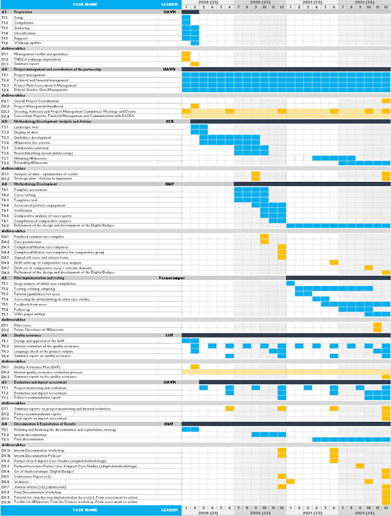
\includegraphics[width=0.72\textwidth]{g.png}
  \caption{Mapa de Gantt (ilustrativo).}
\end{figure}

\subsection{Qualidade da equipa (e do consórcio)}
\begin{campotexto}
\instrucao{Máx. 1000 caracteres}
\end{campotexto}


\section{Orçamento}
\label{sec:orcamento}
% ==============================================================================
% Secção 6: Orçamento
% ==============================================================================

\begin{campotexto}
\instrucao{Descrever resumidamente a visão da equipa quanto ao financiamento do projeto e projeções futuras. Apresentar o quadro resumo dos investimentos do projeto (Tabela~\ref{tab:orcamento}) e fundamentar detalhadamente cada uma das rubricas (Tabela~\ref{tab:fundamentacao_orcamento}). O programa de candidatura define orçamentos entre 1\,M€ e 4\,M€ de financiamento.}
\end{campotexto}

% --- Quadro Resumo Orçamental ---
\begin{table}[H]
\centering\small
\caption{Quadro resumo do orçamento do projeto por rubrica e ano (valores em euros).}
\label{tab:orcamento}
\begin{tabularx}{\textwidth}{Y R{0.13\textwidth} R{0.13\textwidth} R{0.13\textwidth} R{0.15\textwidth}}
  \toprule
  \rowcolor{uatablehead}
  \sffamily\bfseries\textcolor{uadark}{Rubrica de Despesa} &
  \sffamily\bfseries\color{uadark} Ano 1 (€) &
  \sffamily\bfseries\color{uadark} Ano 2 (€) &
  \sffamily\bfseries\color{uadark} Ano 3 (€) &
  \sffamily\bfseries\color{uadark} Total (€) \\
  \midrule
  \sffamily\bfseries Recursos Humanos & 0,00 & 0,00 & 0,00 & \textbf{0,00} \\
  \quad {\footnotesize\color{uamuted} Pessoal técnico, bolseiros e investigadores a contratar} & & & & \\
  \arrayrulecolor{uaborder}\hline
  \sffamily\bfseries Equipamento & 0,00 & 0,00 & 0,00 & \textbf{0,00} \\
  \quad {\footnotesize\color{uamuted} Instrumentos, equipamento científico e \textit{software} específico} & & & & \\
  \hline
  \sffamily\bfseries Matérias-Primas e Componentes & 0,00 & 0,00 & 0,00 & \textbf{0,00} \\
  \quad {\footnotesize\color{uamuted} Consumíveis, materiais de prototipagem e ensaios} & & & & \\
  \hline
  \sffamily\bfseries Participações em Eventos & 0,00 & 0,00 & 0,00 & \textbf{0,00} \\
  \quad {\footnotesize\color{uamuted} Conferências, feiras, divulgação, viagens e estadas} & & & & \\
  \hline
  \sffamily\bfseries Outras Despesas & 0,00 & 0,00 & 0,00 & \textbf{0,00} \\
  \quad {\footnotesize\color{uamuted} Serviços a terceiros, consultoria, propriedade intelectual, etc.} & & & & \\
  \arrayrulecolor{black}\midrule
  \rowcolor{ualightbg}
  \sffamily\bfseries\textcolor{uadark}{Subtotal (Despesas Elegíveis Diretas)} & \textbf{0,00} & \textbf{0,00} & \textbf{0,00} & \textbf{0,00} \\
  \sffamily\bfseries Custos Indiretos (25\%) & 0,00 & 0,00 & 0,00 & \textbf{0,00} \\
  \midrule
  \rowcolor{uatablehead}
  \sffamily\bfseries\textcolor{uadark}{TOTAL GERAL DO PROJETO} & \textbf{0,00} & \textbf{0,00} & \textbf{0,00} & \textbf{0,00} \\
  \bottomrule
\end{tabularx}
\end{table}

% --- Fundamentação de cada rubrica ---
\begin{table}[H]
\centering\small
\caption{Fundamentação das rubricas orçamentais.}
\label{tab:fundamentacao_orcamento}
\begin{tabularx}{\textwidth}{L{0.28\textwidth} Y}
  \toprule
  \rowcolor{uatablehead}
  \sffamily\bfseries\textcolor{uadark}{Rubrica} &
  \sffamily\bfseries\textcolor{uadark}{Fundamentação (critérios de cálculo, quantidades, custos unitários e ligação às tarefas)} \\
  \midrule
  \sffamily\bfseries Recursos Humanos & \instrucao{Justificar perfis, número de pessoas-mês (PM), salários/bolsas de referência e afetação às tarefas do cronograma.} \\ \arrayrulecolor{uaborder}\hline
  \sffamily\bfseries Equipamento & \instrucao{Especificar equipamentos e licenças de \textit{software} necessários, justificar a sua indispensabilidade e indicar valores de mercado ou cotações.} \\ \hline
  \sffamily\bfseries Matérias-Primas e Componentes & \instrucao{Detalhar materiais, componentes de protótipos e consumíveis laboratoriais previstos, associando-os às respetivas tarefas/entregáveis.} \\ \hline
  \sffamily\bfseries Participações em Eventos & \instrucao{Indicar conferências, feiras, demonstrações e deslocações previstas (nacionais e internacionais), estimando inscrições, viagens e alojamento.} \\ \hline
  \sffamily\bfseries Outras Despesas & \instrucao{Fundamentar serviços externos (ensaios especializados, consultoria, patentes, publicações em acesso aberto, auditoria, etc.).} \\ \hline
  \sffamily\bfseries Custos Indiretos (25\%) & \instrucao{Taxa fixa de 25\% sobre as despesas elegíveis diretas para cobertura de custos de estrutura, infraestruturas e gestão administrativa.} \\
  \arrayrulecolor{black}\bottomrule
\end{tabularx}
\end{table}


\section{Referências Bibliográficas}
\label{sec:referencias}
% ==============================================================================
% Secção 7: Referências Bibliográficas
% ==============================================================================

\begin{campotexto}
\instrucao{As referências bibliográficas devem ser geridas no ficheiro {\sffamily referencias.bib} e citadas ao longo do texto com o comando {\sffamily\textbackslash cite\{chave\}} (ex.: \cite{exemplo_artigo2025}). Antes da entrega final, remover o comando {\sffamily\textbackslash nocite\{*\}} abaixo e as entradas ilustrativas de exemplo.}
\end{campotexto}

% Remover \nocite{*} quando o relatório tiver citações reais no texto
\nocite{*}

\bibliographystyle{unsrtnat}
\bibliography{referencias}


\section{Declaração de Uso de Inteligência Artificial}
\label{sec:declaracao_ia}
% ==============================================================================
% Secção 8: Declaração de Uso de Inteligência Artificial
% ==============================================================================

\begin{campotexto}
\instrucao{Os autores devem declarar de forma transparente qualquer utilização de ferramentas de Inteligência Artificial (IA) generativa na preparação desta proposta (ex.: revisão linguística, estruturação, pesquisa exploratória, apoio a código/LaTeX ou geração de elementos visuais). Assinalar a opção aplicável e preencher as tabelas seguintes. Caso não tenham sido utilizadas ferramentas de IA, assinalar a primeira opção e remover as tabelas.}
\end{campotexto}

\noindent\textbf{Declaração de utilização:} (assinalar com $\boxtimes$ a opção aplicável)
\begin{itemize}[leftmargin=1.4em, itemsep=3pt, topsep=4pt]
  \item[$\square$] Os autores declaram que \textbf{não utilizaram} ferramentas de Inteligência Artificial generativa na elaboração deste documento.
  \item[$\square$] Os autores declaram que \textbf{utilizaram} ferramentas de Inteligência Artificial generativa como apoio à elaboração deste documento, nos termos detalhados nas tabelas seguintes, assumindo total responsabilidade pela exatidão científica, originalidade, integridade e revisão crítica de todo o conteúdo apresentado.
\end{itemize}

\subsection{Ferramentas, modelos e finalidade de utilização}

\begin{table}[H]
\centering\small
\caption{Registo das ferramentas e modelos de IA utilizados na elaboração da proposta.}
\label{tab:modelos_ia}
\begin{tabularx}{\textwidth}{L{0.20\textwidth} L{0.13\textwidth} L{0.12\textwidth} L{0.26\textwidth} Y}
  \toprule
  \rowcolor{uatablehead}
  \sffamily\bfseries\textcolor{uadark}{Ferramenta / Modelo (versão)} &
  \sffamily\bfseries\textcolor{uadark}{Data(s)} &
  \sffamily\bfseries\textcolor{uadark}{Secção(ões)} &
  \sffamily\bfseries\textcolor{uadark}{Finalidade / Tarefa} &
  \sffamily\bfseries\textcolor{uadark}{Validação humana efetuada} \\
  \midrule
  \instrucao{Ex.: ChatGPT (GPT-4o)} & \instrucao{dd/mm/aaaa} & \instrucao{Sec. 2 e 3} & \instrucao{Revisão linguística, clareza e síntese do resumo em inglês.} & \instrucao{Verificação integral da terminologia técnica e fidelidade ao texto original.} \\ \arrayrulecolor{uaborder}\hline
  \instrucao{Ex.: Gemini (2.5 Pro)} & \instrucao{dd/mm/aaaa} & \instrucao{Sec. 5 e 6} & \instrucao{Apoio à estruturação de tabelas LaTeX e verificação de consistência.} & \instrucao{Revisão manual de todos os valores, fórmulas e código LaTeX.} \\ \hline
  & & & & \\
  \arrayrulecolor{black}\bottomrule
\end{tabularx}
\end{table}

\subsection{Registo dos \textit{prompts} utilizados}

\begin{table}[H]
\centering\small
\caption{Registo dos principais \textit{prompts} submetidos e respetiva integração no documento.}
\label{tab:prompts_ia}
\begin{tabularx}{\textwidth}{L{0.16\textwidth} L{0.11\textwidth} L{0.40\textwidth} Y}
  \toprule
  \rowcolor{uatablehead}
  \sffamily\bfseries\textcolor{uadark}{ID / Modelo} &
  \sffamily\bfseries\textcolor{uadark}{Secção} &
  \sffamily\bfseries\textcolor{uadark}{\textit{Prompt} utilizado (texto ou síntese fiel)} &
  \sffamily\bfseries\textcolor{uadark}{Alterações e validação pelos autores} \\
  \midrule
  \instrucao{P1 -- GPT-4o} & \instrucao{Sec. 2.2} & \instrucao{``Melhora a fluidez académica em inglês do seguinte resumo técnico mantendo todos os dados quantitativos: [\ldots]''} & \instrucao{Ajustados termos técnicos de engenharia mecânica e reduzido para cumprir o limite de 1000 caracteres.} \\ \arrayrulecolor{uaborder}\hline
  \instrucao{P2 -- Gemini} & \instrucao{Sec. 6} & \instrucao{``Cria uma tabela em LaTeX com booktabs para distribuir cinco rubricas orçamentais por três anos.''} & \instrucao{Adaptadas as colunas, rubricas e preenchidos todos os valores com base nas cotações da equipa.} \\ \hline
  & & & \\
  \arrayrulecolor{black}\bottomrule
\end{tabularx}
\end{table}

\subsection{Conformidade ética, confidencialidade e integridade científica}

\begin{itemize}[leftmargin=1.4em, itemsep=4pt, topsep=4pt]
  \item \textbf{Autonomia e autoria:} As ferramentas de IA não são consideradas coautoras; todas as decisões científicas, metodológicas e de redação final pertencem exclusivamente aos autores.
  \item \textbf{Verificação de factos e referências:} Todos os dados quantitativos, equações, normas e referências bibliográficas incluídos no relatório foram verificados diretamente nas fontes originais, garantindo a ausência de citações inexistentes ou imprecisões.
  \item \textbf{Privacidade e propriedade intelectual:} Não foram submetidos em plataformas públicas de IA dados pessoais, informação confidencial de parceiros industriais ou conteúdos protegidos por acordos de confidencialidade (NDA).
\end{itemize}



% --- Nota final de entrega ---
\vspace{1.2cm}
\noindent\textcolor{uaborder}{\rule{\textwidth}{0.6pt}}
\par\vspace{4pt}
{\sffamily\footnotesize\color{uamuted}\textit{A versão final deste documento deve ser entregue em PDF. Eventuais anexos deverão ser incluídos no mesmo formato.}}

\end{document}
